\part{Filosofia}
\label{ch:philosophy}
\chapter*{Filosofia}

\begin{chapquote}{Lewis Carroll, \textit{Alice no País das Maravilhas}}
O camundongo lançou-lhe um olhar um tanto inquisitivo, pareceu piscar um olho, mas não disse nada.
\end{chapquote}

Olhando para o Bitcoin superficialmente, alguém pode concluir que ele é lento, custoso, redundante demais e excessivamente paranóico. Olhando para o Bitcoin com curiosidade pode-se descobrir que as coisas não são o que parecem ser à primeira vista.

O Bitcoin tem uma maneira de pegar as suposições e transformá-las em nossas cabeças. Depois de um tempo, quando você estava prestes a se sentir confortável de novo, o Bitcoin se destrói na parede como um touro em uma loja de porcelana e destruirá suas suposições mais uma vez.

\begin{figure}
  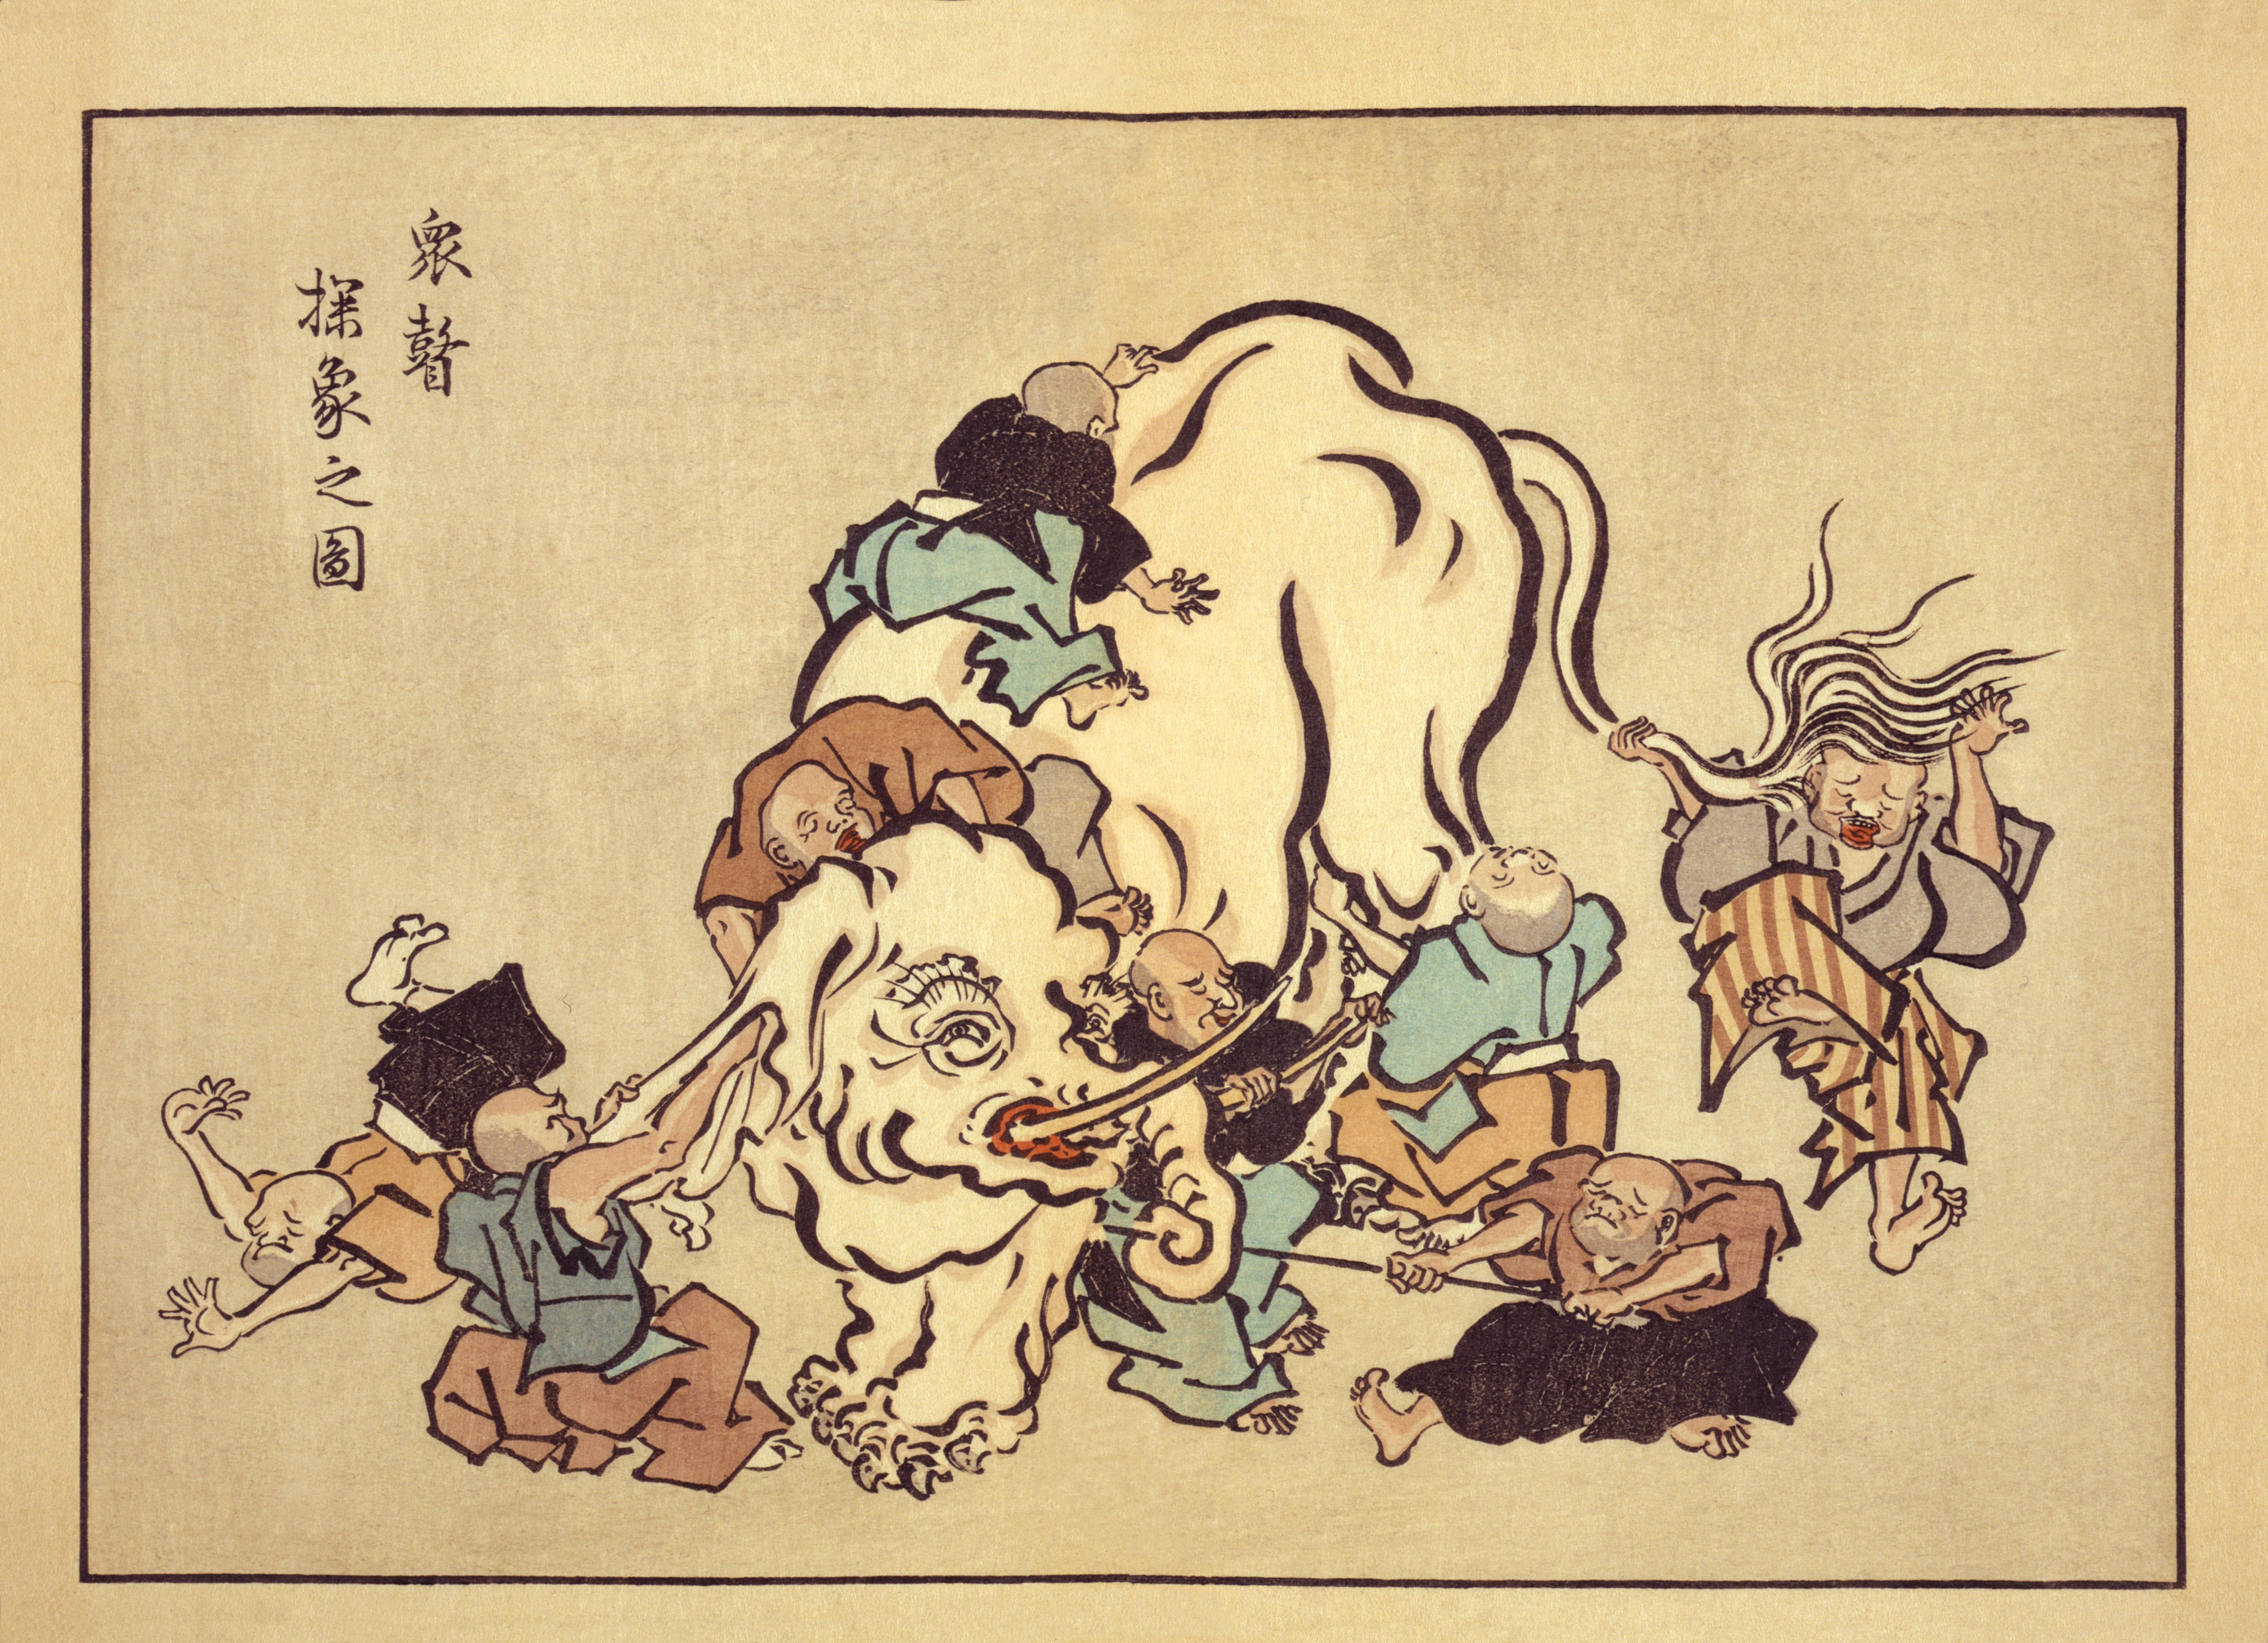
\includegraphics{assets/images/blind-monks.jpg}
  \caption{Monges cegos examinando o Touro Bitcoin}
  \label{fig:blind-monks}
\end{figure}

O Bitcoin é filho de muitas disciplinas. Como monges cegos examinando um elefante, todos os que abordam essa nova tecnologia o fazem de um ângulo diferente. E todos chegarão a conclusões diferentes sobre a natureza dessa fera.

As lições a seguir são sobre algumas das minhas suposições que o Bitcoin destruiu e as conclusões que acabei encontrando. Questões filosóficas de imutabilidade, escassez, localidade e identidade são exploradas nas primeiras quatro lições. Cada parte consiste em sete lições.

~

\begin{samepage}
Parte~\ref{ch:philosophy} -- \nameref{ch:philosophy}:

\begin{enumerate}
  \item \nameref{les:1}
  \item \nameref{les:2}
  \item \nameref{les:3}
  \item \nameref{les:4}
  \item \nameref{les:5}
  \item \nameref{les:6}
  \item \nameref{les:7}
\end{enumerate}
\end{samepage}

A lição \ref{les:5} explora como a história de origem do Bitcoin não é apenas fascinante, mas absolutamente essencial para um sistema sem governante ou líder. As duas últimas lições deste capítulo exploram o poder da liberdade de expressão e os limites de nosso conhecimento individual, refletidos pela surpreendente profundidade da toca do coelho do Bitcoin.

Espero que você ache o mundo do Bitcoin tão educativo, fascinante e divertido quanto eu achei e ainda acho. Convido você a seguir o coelho e explorar as profundezas desta toca do coelho. Agora segure seu relógio de bolso, desça e aproveite a queda.